Tools were run on the function \texttt{send\_publish\_notifications(..)} and on the file \texttt{tools.py}.

\paragraph{Pylint}
The Python quality checker \emph{Pylint} is a tool to help with coding standard as recommended by PEP 8, error detection and refactoring.
Pylint message categories:
\begin{itemize}
    \item (C) convention: programming standard violation
    \item (R) refactor: code smell
    \item (W) warning: python specific problem
    \item (E) error: likely bug
    \item (F) fatal: an error occurred preventing pylint from continuing the analysis
\end{itemize}
\begin{figure}[h]
    \centering
    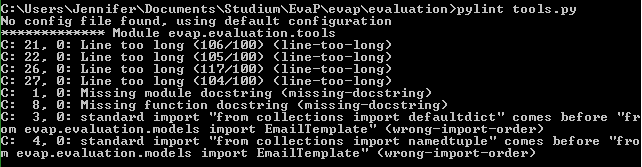
\includegraphics[width=\textwidth, keepaspectratio]{graphics/pylint_send_publish_notifications_1}
    \caption{Pylint messages for \texttt{send\_publish\_notifications(..)}}
    \label{fig:pylint}
\end{figure} 
As expected after our testing Pylint found mostly violated coding conventions in \texttt{send\_publish\_notifications(..)} (\ref{fig:pylint}). 
The investigation of the file \texttt{tools.py} leads to a few warnings and refactoring hints that we will discuss with the developers on the next occasion.
%TODO Restliche Grafiken in den Anhang?


\paragraph{PyCharm}

\paragraph{Pychecker}
% Does not support 
% length of each line
% variable names (well-formed)
% implementation of declared interfaces

\paragraph{Pyflakes}

\paragraph{Landscape}
